\documentclass[aspectratio=169,10pt]{beamer}

\usepackage[utf8]{inputenc}
\usepackage{amsmath, amssymb, amsfonts, amsthm}
\usepackage{mathtools}
\usepackage{graphicx}
\usepackage{hyperref}
\usepackage{listings}
\usepackage{xcolor}
\usepackage{geometry}

% Theme and color scheme
\usetheme{Madrid}
\usecolortheme{seahorse}

% Set up listings style for code
\lstset{
    basicstyle=\ttfamily\scriptsize,
    commentstyle=\color{green!50!black}\itshape,
    keywordstyle=\color{blue}\bfseries,
    stringstyle=\color{red},
    breaklines=true,
    frame=single,
    numbers=left,
    numberstyle=\tiny\color{gray},
    showstringspaces=false
}

% Graphics path
\graphicspath{{figures/}}

% Footer with slide numbers
\setbeamertemplate{footline}[frame number]

% Title page information
\title{Measurable Selections of Multifunctions}
\subtitle{Chapter 10c: Applications of Fixed Point Theorems for Multifunctions}
\author{Based on Pathak's \textit{An Introduction to Nonlinear Analysis and Fixed Point Theory}}
\date{}
\institute{}

\begin{document}

% ============================================================================
% TITLE SLIDE
% ============================================================================
\begin{frame}
\titlepage
\end{frame}

% ============================================================================
% OUTLINE
% ============================================================================
\begin{frame}{Outline}
\tableofcontents
\end{frame}

% ============================================================================
% SECTION 1: FOUNDATIONAL CONCEPTS
% ============================================================================
\section{Foundational Concepts}

\begin{frame}{Measure Spaces and Measurability}
\begin{definition}[Measure Space]
A \textbf{measure space} is a triple $(\Omega, \mathcal{A}, \mu)$ where:
\begin{itemize}
    \item $\Omega$ is a nonempty set (sample space)
    \item $\mathcal{A}$ is a $\sigma$-algebra of subsets of $\Omega$
    \item $\mu: \mathcal{A} \to [0, \infty]$ is a \textbf{measure} (countably additive function)
\end{itemize}
\end{definition}

\vspace{0.3cm}

\begin{definition}[$\sigma$-algebra]
A collection $\mathcal{A}$ of subsets of $\Omega$ is a $\sigma$-algebra if:
\begin{enumerate}
    \item $\emptyset, \Omega \in \mathcal{A}$
    \item If $A \in \mathcal{A}$, then $A^c \in \mathcal{A}$ (closed under complements)
    \item If $\{A_n\}_{n=1}^{\infty} \subseteq \mathcal{A}$, then $\bigcup_{n=1}^{\infty} A_n \in \mathcal{A}$ (closed under countable unions)
\end{enumerate}
\end{definition}
\end{frame}

\begin{frame}{Measure Space Structure}
\begin{center}
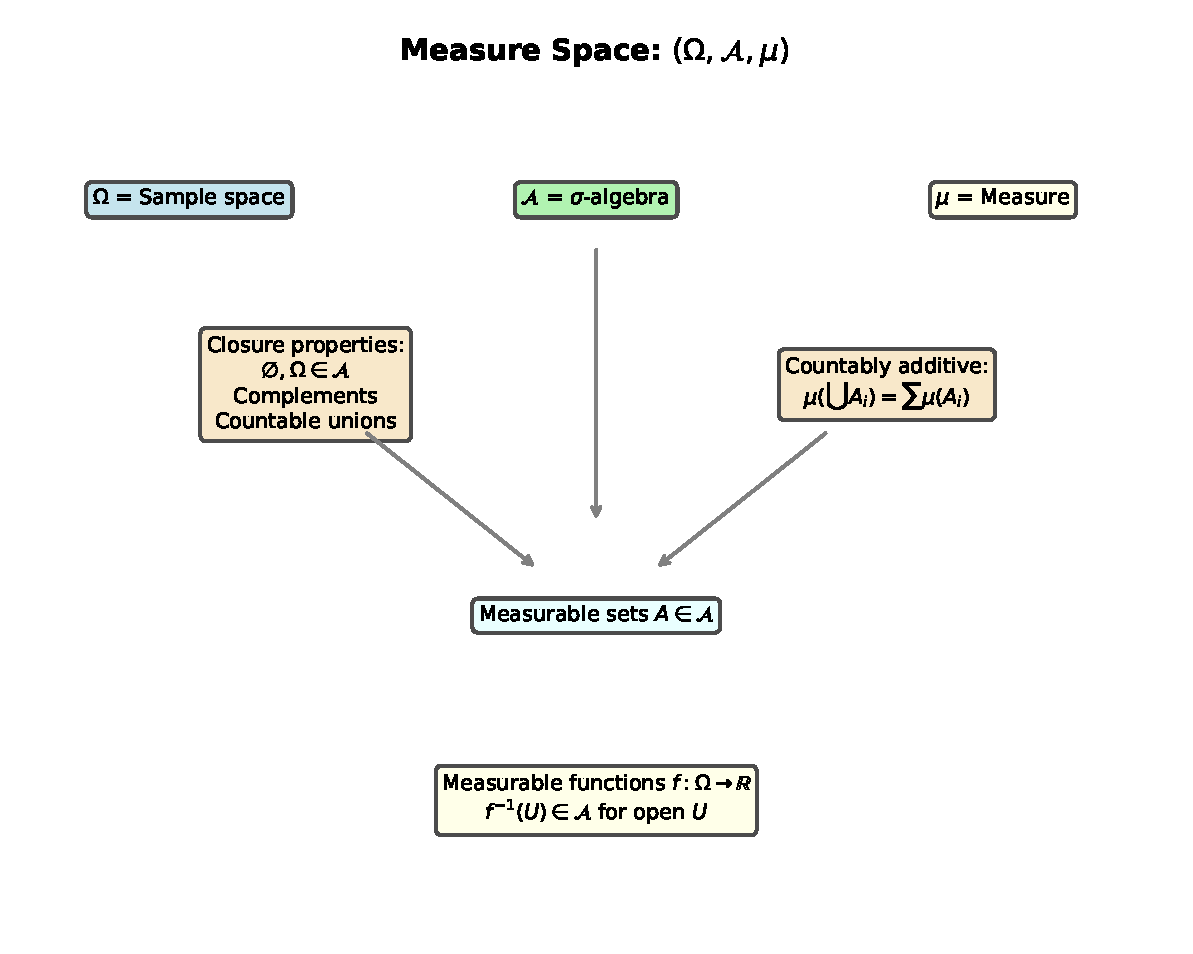
\includegraphics[width=0.85\textwidth]{measure_space_structure.pdf}
\end{center}

\vspace{-0.3cm}
\begin{remark}
\begin{itemize}
    \item Elements of $\mathcal{A}$ are called \textbf{measurable sets}
    \item A finite measure space has $\mu(\Omega) < \infty$
    \item A $\sigma$-finite measure space is a countable union of finite measure sets
\end{itemize}
\end{remark}
\end{frame}

\begin{frame}{Measurable Functions}
\begin{definition}[Measurable Function]
Let $(\Omega, \mathcal{A})$ be a measurable space and $(Y, \mathcal{V})$ be a topological space. A mapping $f: \Omega \to Y$ is \textbf{measurable} if
$$f^{-1}(V) \in \mathcal{A} \quad \text{for every open set } V \subseteq Y.$$
\end{definition}

\vspace{0.3cm}

\begin{theorem}[Properties of Measurable Functions]
If $f, g: \Omega \to \mathbb{R}$ are measurable functions, then:
\begin{enumerate}
    \item $f + g, \, f - g, \, f \cdot g$ are measurable
    \item $|f|, \, f^+, \, f^-$ are measurable
    \item $\sup_n f_n, \, \inf_n f_n, \, \limsup_n f_n$ are measurable (if limits exist)
\end{enumerate}
\end{theorem}
\end{frame}

\begin{frame}{Simple Functions}
\begin{definition}[Simple Function]
A function $s: \Omega \to [0, \infty)$ is \textbf{simple} if its range is a finite set. If $c_1, c_2, \ldots, c_n$ are the distinct values and
$$E_i = \{x \in \Omega: s(x) = c_i\}, \quad i = 1, 2, \ldots, n,$$
then
$$s(x) = \sum_{i=1}^{n} c_i \chi_{E_i}(x),$$
where $\chi_{E_i}$ is the characteristic function of $E_i$.
\end{definition}

\vspace{0.3cm}

\begin{theorem}[Approximation by Simple Functions]
Let $u: \Omega \to [0, \infty)$ be a measurable function. There exists a sequence $\{u_n\}$ of simple functions such that:
\begin{enumerate}
    \item $0 \le u_1(x) \le u_2(x) \le \cdots \le u(x)$ for all $x \in \Omega$
    \item $u_n(x) \to u(x)$ as $n \to \infty$ for all $x \in \Omega$
\end{enumerate}
\end{theorem}
\end{frame}

% ============================================================================
% SECTION 2: MULTIFUNCTIONS
% ============================================================================
\section{Multifunctions}

\begin{frame}{Multifunctions: Definition and Basics}
\begin{definition}[Multifunction]
Let $X$ and $Y$ be nonempty sets. A \textbf{multifunction} (or set-valued map) is a mapping
$$F: X \to \mathcal{P}(Y),$$
where $\mathcal{P}(Y)$ denotes the power set (family of all subsets of $Y$).

For each $x \in X$, the image $F(x) \subseteq Y$ is the set of all possible values associated with $x$.
\end{definition}

\vspace{0.3cm}

\begin{example}
\begin{itemize}
    \item $F: \mathbb{R} \to \mathcal{P}(\mathbb{R})$ defined by $F(x) = \{y \in \mathbb{R}: y^2 = x\}$
    \item Correspondence in economics: price set $\to$ demand bundles
    \item Differential inclusion: $x'(t) \in F(t, x(t))$
\end{itemize}
\end{example}
\end{frame}

\begin{frame}{Multifunction Illustration}
\begin{center}
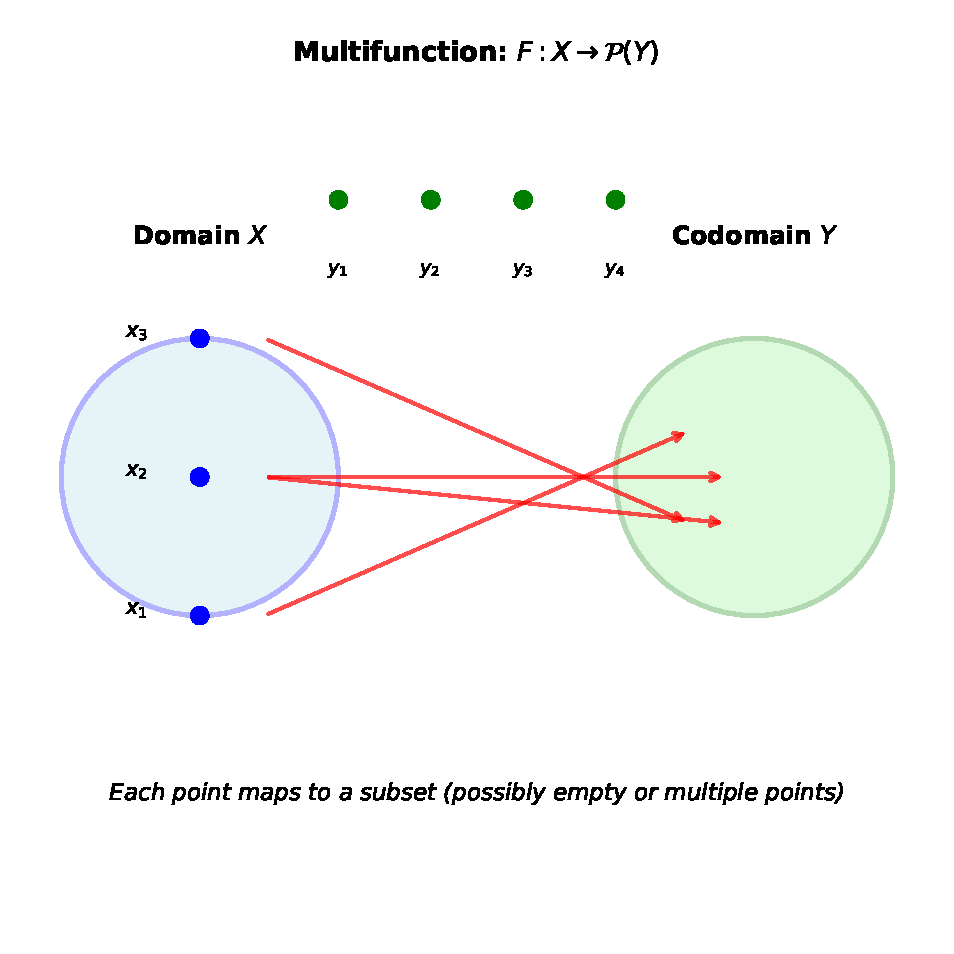
\includegraphics[width=0.85\textwidth]{multifunction.pdf}
\end{center}

\vspace{0.2cm}
\begin{remark}
A standard function is a special case where $|F(x)| = 1$ for each $x$.
\end{remark}
\end{frame}

\begin{frame}{Types of Multifunctions}
\begin{definition}
A multifunction $F: X \to \mathcal{P}(Y)$ is said to have:
\begin{itemize}
    \item \textbf{Closed values} if $F(x)$ is a closed set for every $x \in X$
    \item \textbf{Convex values} if $F(x)$ is a convex set for every $x \in X$
    \item \textbf{Compact values} if $F(x)$ is a compact set for every $x \in X$
    \item \textbf{Nonempty values} if $F(x) \neq \emptyset$ for every $x \in X$
\end{itemize}
\end{definition}

\vspace{0.3cm}

\begin{definition}[Graph of a Multifunction]
The \textbf{graph} of $F: X \to \mathcal{P}(Y)$ is defined as
$$\text{Graph}(F) = \{(x, y) \in X \times Y: y \in F(x)\}.$$
\end{definition}
\end{frame}

\begin{frame}{Hausdorff Distance}
\begin{definition}[Hausdorff Distance]
For nonempty subsets $A, B$ of a metric space $(Y, d)$, the \textbf{Hausdorff distance} is
$$H(A, B) = \max\left\{\sup_{a \in A} d(a, B), \sup_{b \in B} d(b, A)\right\},$$
where $d(a, B) = \inf_{b \in B} d(a, b)$.
\end{definition}

\vspace{0.3cm}

\begin{remark}
\begin{itemize}
    \item $H$ defines a metric on the space of nonempty compact sets
    \item Useful for measuring the distance between image sets
    \item Essential for studying continuity of multifunctions
\end{itemize}
\end{remark}
\end{frame}

% ============================================================================
% SECTION 3: MEASURABLE SELECTIONS
% ============================================================================
\section{Measurable Selections}

\begin{frame}{Selection Functions}
\begin{definition}[Selection]
Let $F: X \to \mathcal{P}(Y)$ be a multifunction. A function $f: X \to Y$ is called a \textbf{selection} (or \textbf{selector}) of $F$ if
$$f(x) \in F(x) \quad \text{for all } x \in X.$$
\end{definition}

\vspace{0.3cm}

\begin{example}
For $F(x) = \{y \in \mathbb{R}: |y| \le x\}$:
\begin{itemize}
    \item $f_1(x) = x$ is a selection
    \item $f_2(x) = -x$ is a selection
    \item $f_3(x) = \frac{x}{2}$ is a selection
\end{itemize}
\end{example}
\end{frame}

\begin{frame}{Selection Function Illustration}
\begin{center}
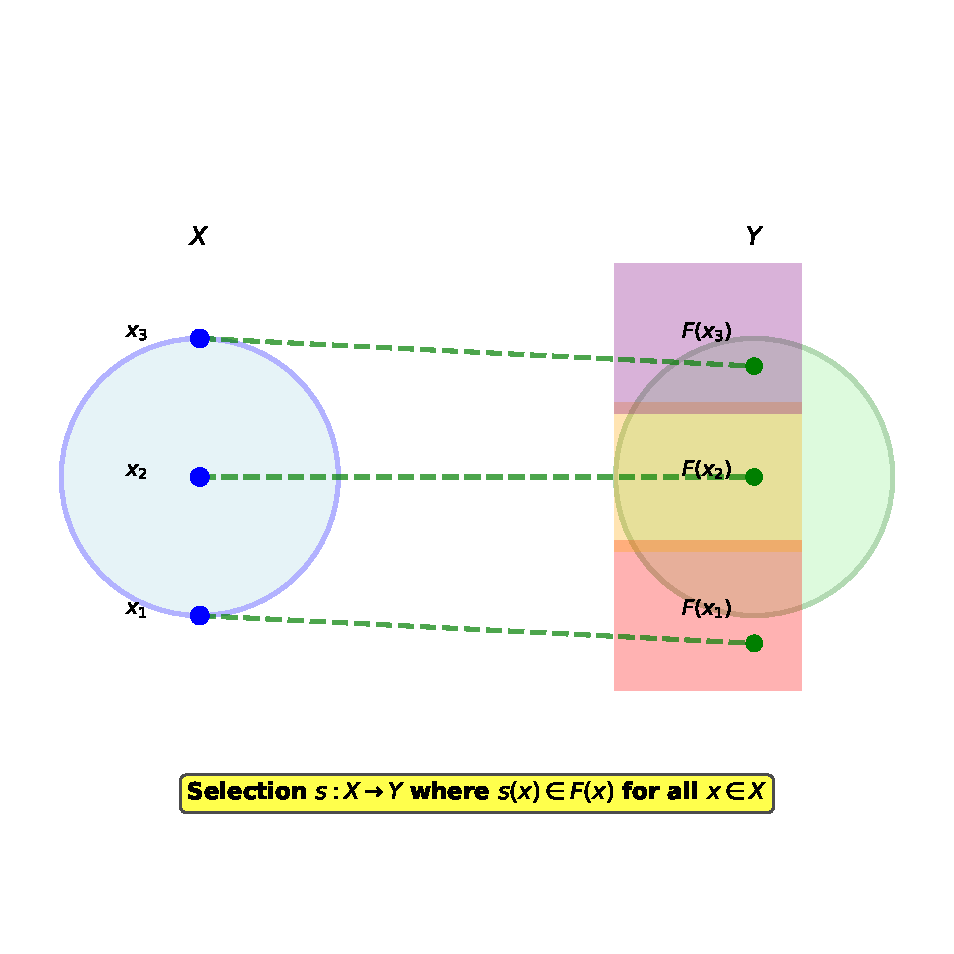
\includegraphics[width=0.85\textwidth]{selection_function.pdf}
\end{center}
\end{frame}

\begin{frame}{Measurable Selections}
\begin{definition}[Measurable Selection]
Let $(\Omega, \mathcal{A}, \mu)$ be a measure space, $X$ a separable Banach space, and $F: \Omega \to \mathcal{P}(X)$ a multifunction.

A measurable function $s: \Omega \to X$ is a \textbf{measurable selection} of $F$ if:
\begin{enumerate}
    \item $s(\omega) \in F(\omega)$ for $\mu$-almost every $\omega \in \Omega$
    \item $s$ is (Borel) measurable with respect to $\mathcal{A}$ and the Borel $\sigma$-algebra of $X$
\end{enumerate}
\end{definition}

\vspace{0.3cm}

\begin{remark}
Measurable selections are crucial for:
\begin{itemize}
    \item Proving existence of solutions to integral and differential inclusions
    \item Establishing measurability properties of dependent choices
    \item Optimal control and variational problems
\end{itemize}
\end{remark}
\end{frame}

\begin{frame}{Measurability of Multifunctions}
\begin{definition}[Measurable Multifunction]
A multifunction $F: \Omega \to \mathcal{P}(Y)$ (with $\Omega$ a measure space and $Y$ a separable Banach space) is said to be:

\begin{itemize}
    \item \textbf{Weakly measurable} if for each $y \in Y$, the function
    $$\omega \mapsto d(y, F(\omega)) = \inf_{f \in F(\omega)} \|y - f\|$$
    is measurable.

    \item \textbf{Strongly measurable} if there exist measurable selections $s_n: \Omega \to Y$ such that
    $$F(\omega) = \overline{\{s_n(\omega): n \in \mathbb{N}\}} \text{ for a.e. } \omega.$$
\end{itemize}
\end{definition}
\end{frame}

\begin{frame}{Measurability Conditions}
\begin{theorem}[Measurability Equivalent Conditions]
For a multifunction $F: \Omega \to \mathcal{P}(Y)$ with $(\Omega, \mathcal{A}, \mu)$ a measure space and $Y$ a separable Banach space:

\begin{enumerate}
    \item $F^{-1}(U) := \{\omega \in \Omega: F(\omega) \cap U \neq \emptyset\} \in \mathcal{A}$ for all open $U \subseteq Y$
    \item For each closed $C \subseteq Y$, we have $F^{-1}_c(C) := \{\omega: F(\omega) \subseteq C\} \in \mathcal{A}$
    \item $F$ admits a countable family of measurable selections $\{f_n\}$ such that
    $$F(\omega) = \overline{\{f_n(\omega): n \in \mathbb{N}\}} \text{ for a.e. } \omega \in \Omega.$$
\end{enumerate}

These conditions are equivalent when $F$ has closed, nonempty values.
\end{theorem}
\end{frame}

\begin{frame}{Measurability Illustration}
\begin{center}
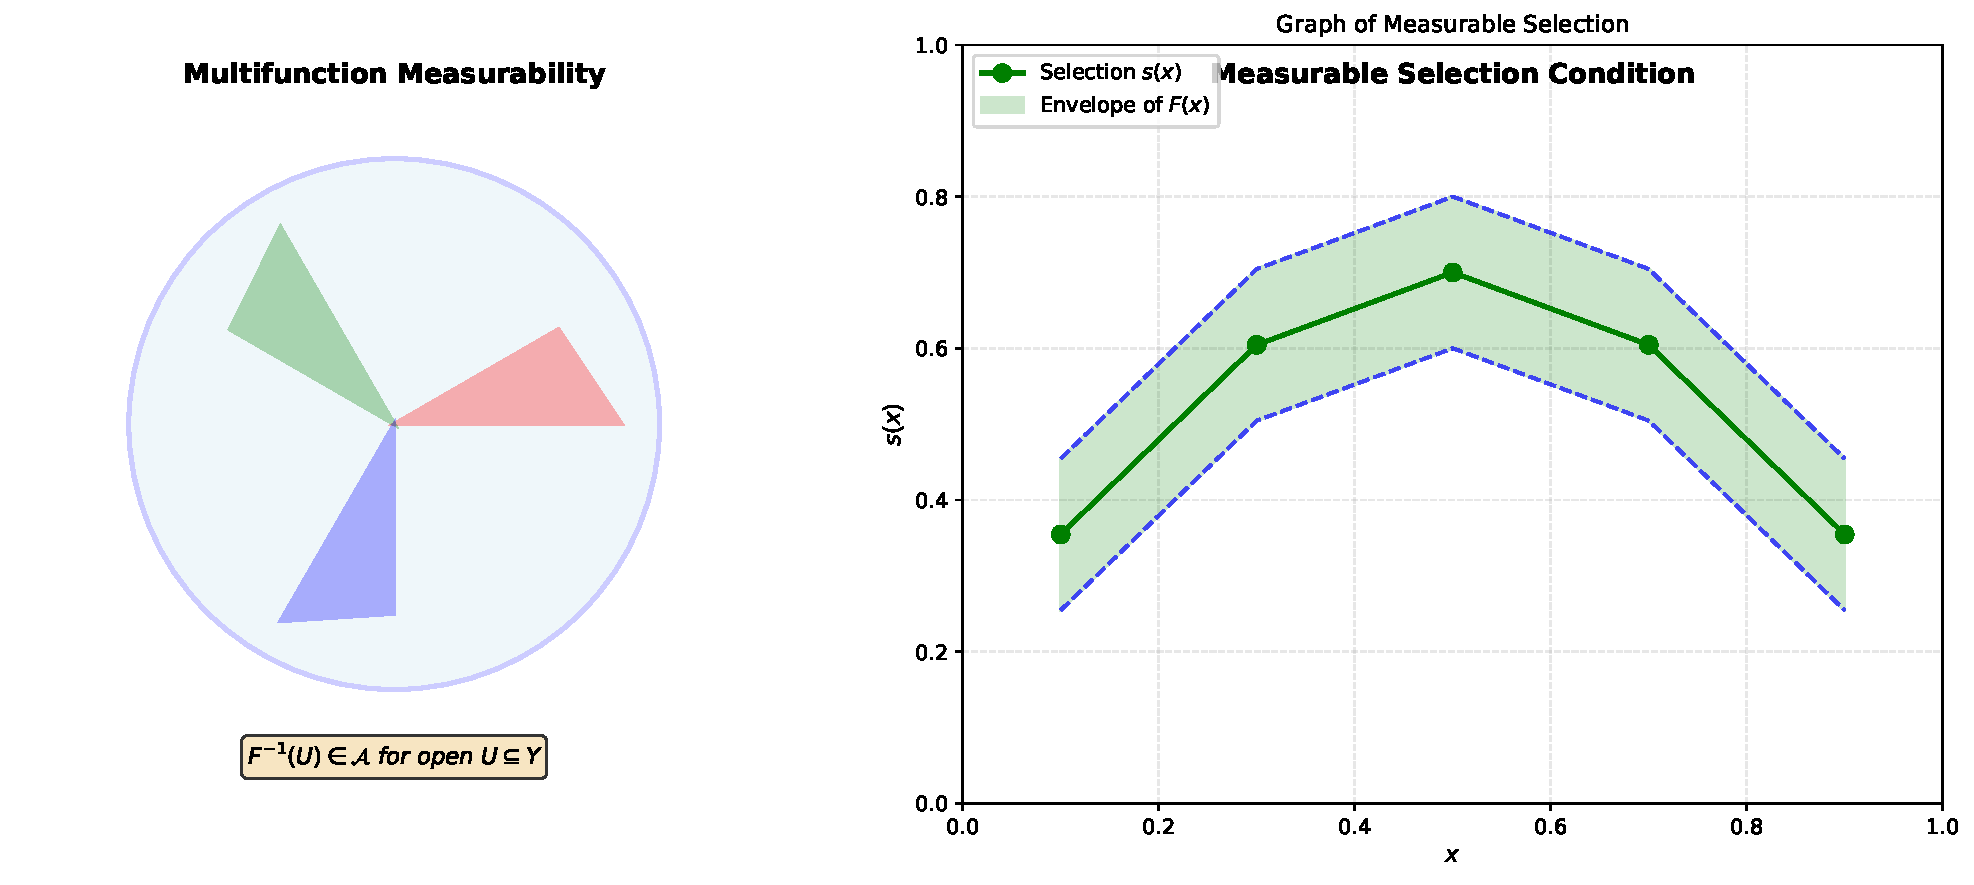
\includegraphics[width=0.85\textwidth]{measurability_multifunction.pdf}
\end{center}
\end{frame}

% ============================================================================
% SECTION 4: FILIPOV SELECTION THEOREM
% ============================================================================
\section{Filipov Selection Theorem}

\begin{frame}{Filipov's Selection Theorem}
\begin{theorem}[Filipov Selection Theorem]
Let $(\Omega, \mathcal{A}, \mu)$ be a $\sigma$-finite measure space, $X$ a separable Banach space, and $F: \Omega \times X \to \mathcal{P}(X)$ a multifunction satisfying:

\begin{enumerate}
    \item For each $x \in X$, the multifunction $\omega \mapsto F(\omega, x)$ is measurable
    \item For each $\omega \in \Omega$, $F(\omega, \cdot)$ has closed, nonempty values
    \item For some measurable function $k: \Omega \to \mathbb{R}^+$, the Lipschitz condition holds:
    $$H(F(\omega, x), F(\omega, y)) \le k(\omega) \|x - y\| \quad \text{for all } x, y \in X \text{ and a.e. } \omega$$
\end{enumerate}

Then there exists a measurable selection $s: \Omega \to X$ such that
$$s(\omega) \in F(\omega) \quad \text{for a.e. } \omega \in \Omega.$$
\end{theorem}
\end{frame}

\begin{frame}{Filipov Selection Theorem Illustration}
\begin{center}
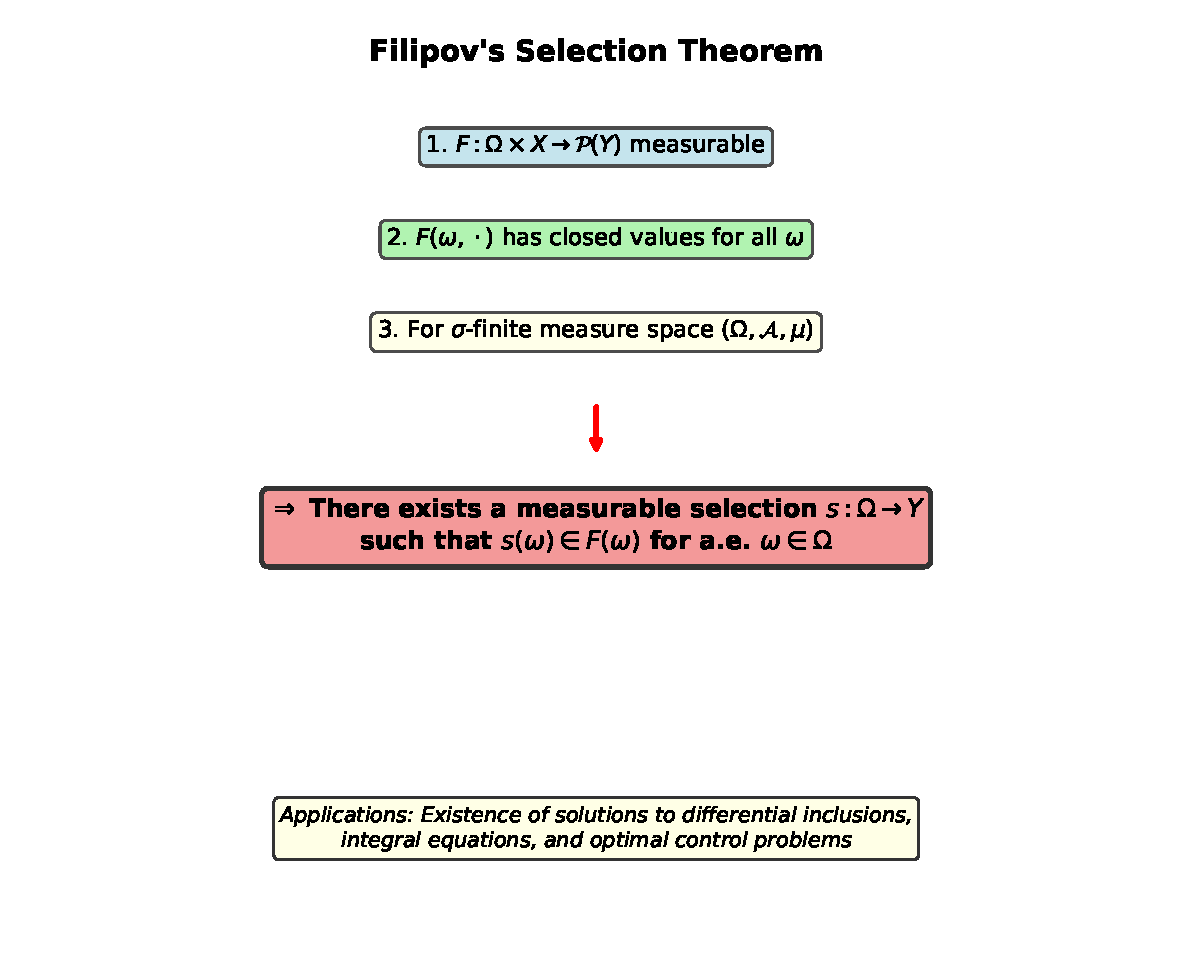
\includegraphics[width=0.85\textwidth]{filipov_selection_theorem.pdf}
\end{center}

\vspace{0.3cm}
\begin{remark}
This is a fundamental result that guarantees the existence of measurable selections under reasonable conditions.
\end{remark}
\end{frame}

\begin{frame}{Applications of Filipov's Theorem}
The Filipov Selection Theorem has important applications:

\begin{enumerate}
    \item \textbf{Differential Inclusions}: Existence of solutions to
    $$x'(t) \in F(t, x(t)), \quad x(0) = x_0$$

    \item \textbf{Integral Inclusions}: Solving
    $$x(t) = \lambda(t) + \int_0^t u(s, x(s)) \, ds, \quad u(s, x) \in F(s, x)$$

    \item \textbf{Optimal Control}: Finding measurable control functions in
    $$\min_{u(t) \in F(t)} \int_0^T g(t, x(t), u(t)) \, dt$$

    \item \textbf{Variational Inequalities}: Proving solvability of structured variational problems
\end{enumerate}
\end{frame}

% ============================================================================
% SECTION 5: BOCHNER INTEGRAL
% ============================================================================
\section{Integration in Banach Spaces}

\begin{frame}{Bochner Integral in Banach Spaces}
\begin{definition}[Strongly Measurable Function]
A function $u: \Omega \to X$ (where $X$ is a Banach space) is \textbf{strongly measurable} if there exists a sequence $\{u_n\}$ of simple functions such that
$$\|u_n(x) - u(x)\|_X \to 0 \quad \text{as } n \to \infty \text{ for a.e. } x \in \Omega.$$
\end{definition}

\vspace{0.3cm}

\begin{definition}[Bochner Integrable]
A strongly measurable function $u: \Omega \to X$ is \textbf{Bochner integrable} if there exists a sequence of simple functions $\{u_n\}$ such that
$$\int_\Omega \|u_n(\omega) - u(\omega)\|_X \, d\mu(\omega) \to 0 \quad \text{as } n \to \infty.$$
\end{definition}
\end{frame}

\begin{frame}{Bochner Integral Definition}
\begin{definition}[Bochner Integral]
For a Bochner integrable function $u: \Omega \to X$, the \textbf{Bochner integral} is defined as
$$\int_E u \, d\mu = \lim_{n \to \infty} \int_E u_n \, d\mu,$$
where $\{u_n\}$ is a sequence of simple functions converging to $u$ in the sense above, and $E \in \mathcal{A}$.
\end{definition}

\vspace{0.3cm}

\begin{remark}
The limit is independent of the choice of approximating simple functions.
\end{remark}
\end{frame}

\begin{frame}{Bochner Integral Illustration}
\begin{center}
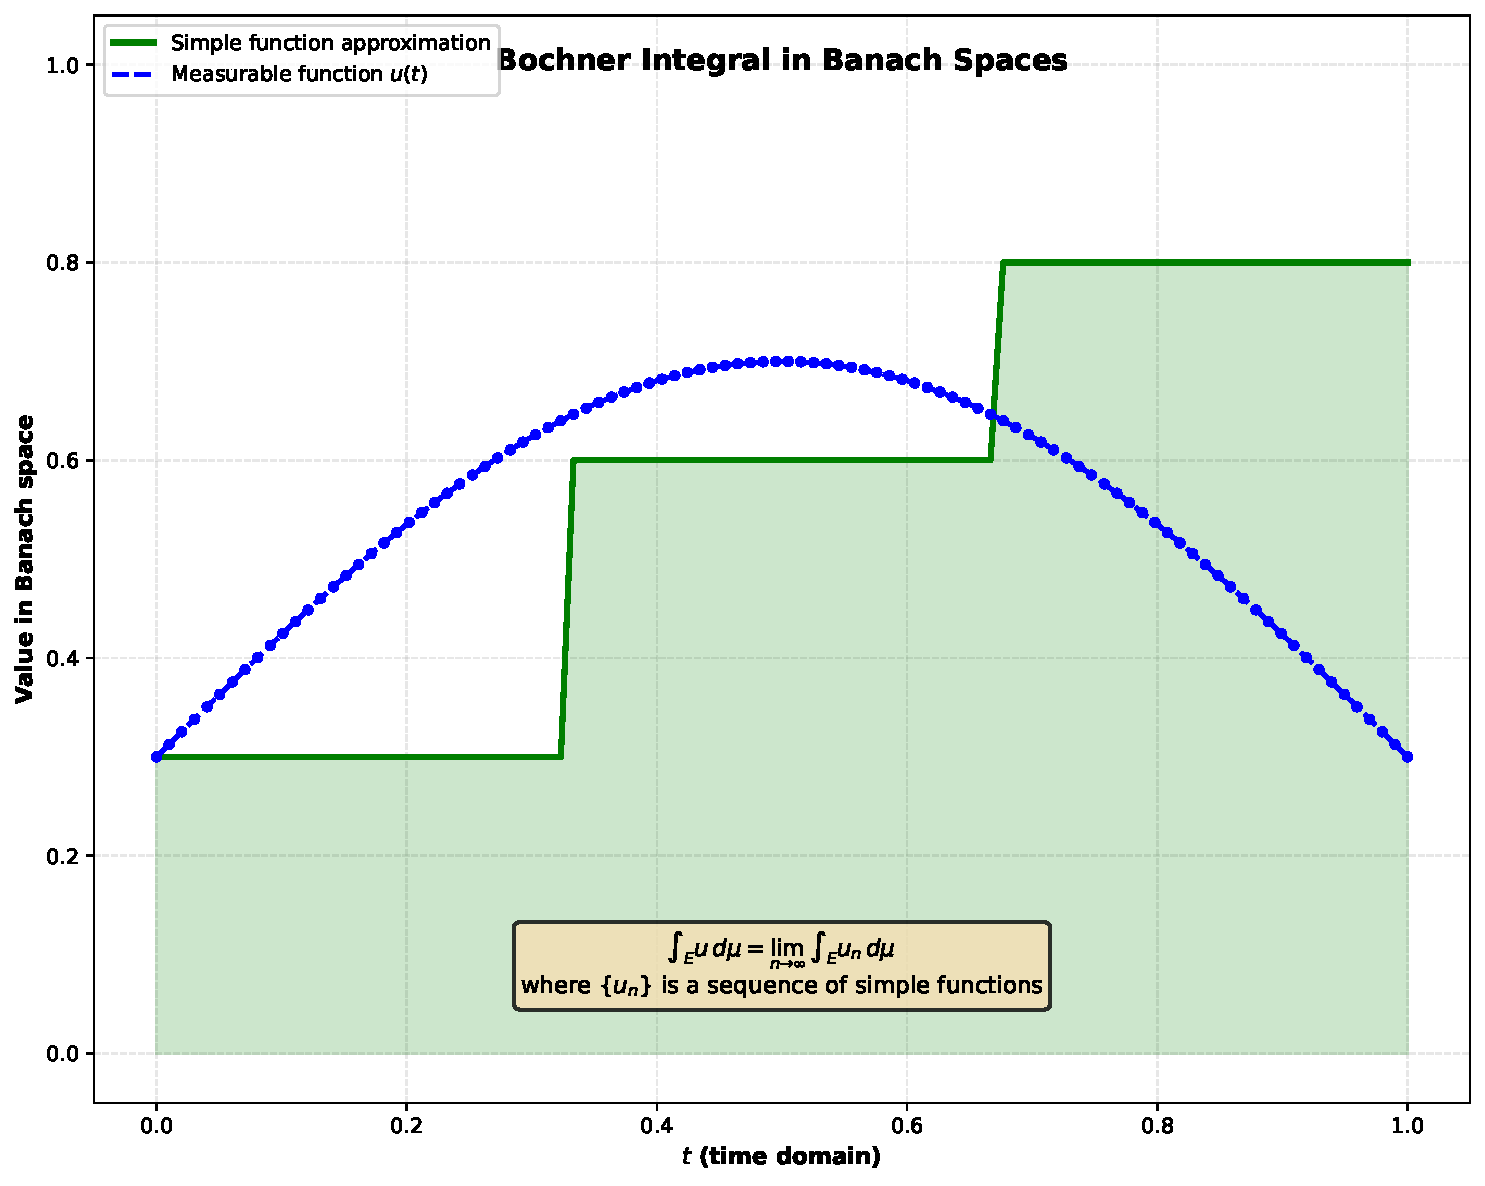
\includegraphics[width=0.90\textwidth]{bochner_integral.pdf}
\end{center}
\end{frame}

\begin{frame}{Properties of Bochner Integral}
\begin{theorem}[Properties of Bochner Integral]
Let $u, v: \Omega \to X$ be Bochner integrable. Then:

\begin{enumerate}
    \item \textbf{Linearity}: For $a, b \in \mathbb{R}$,
    $$\int_E (au + bv) \, d\mu = a \int_E u \, d\mu + b \int_E v \, d\mu$$

    \item \textbf{Countable Additivity}: If $\{E_n\}$ is a countable partition of $E$,
    $$\int_E u \, d\mu = \sum_{n=1}^\infty \int_{E_n} u \, d\mu$$

    \item \textbf{Norm estimate}:
    $$\left\|\int_E u \, d\mu\right\|_X \le \int_E \|u\|_X \, d\mu$$

    \item \textbf{Dominated Convergence}: If $\|u_n\| \le g$ for a $\mu$-integrable $g$, then
    $$\int_E u_n \, d\mu \to \int_E u \, d\mu \quad \text{as } n \to \infty$$
\end{enumerate}
\end{theorem}
\end{frame}

% ============================================================================
% SECTION 6: APPLICATIONS
% ============================================================================
\section{Applications}

\begin{frame}{Existence of Solutions to Differential Inclusions}
\begin{theorem}[Existence for Differential Inclusions]
Let $X$ be a separable Banach space, $[a, b]$ a compact interval, and $F: [a, b] \times X \to \mathcal{P}(X)$ a multifunction satisfying:

\begin{enumerate}
    \item $F(t, \cdot)$ is measurable for each $x \in X$
    \item $F(\cdot, x)$ has closed, convex values for each $x \in X$
    \item $\|F(t, x)\| := \sup_{v \in F(t,x)} \|v\| \le M(t)(1 + \|x\|)$ for some integrable $M: [a,b] \to \mathbb{R}^+$
\end{enumerate}

Then for any $x_0 \in X$, there exists an absolutely continuous solution
$$x: [a, b] \to X, \quad x(a) = x_0,$$
to the differential inclusion
$$\frac{dx}{dt} \in F(t, x(t)) \quad \text{for a.e. } t \in [a, b].$$
\end{theorem}
\end{frame}

\begin{frame}{Integral Inclusions}
\begin{definition}[Integral Inclusion]
An \textbf{integral inclusion} has the form
$$x(t) \in \lambda(t) + \int_0^t F(s, x(s)) \, ds, \quad t \in [0, T],$$
where:
\begin{itemize}
    \item $\lambda: [0, T] \to X$ is continuous
    \item $F: [0, T] \times X \to \mathcal{P}(X)$ is a measurable multifunction
    \item The integral is understood in the Bochner sense
\end{itemize}
\end{definition}

\vspace{0.3cm}

\begin{theorem}[Existence for Integral Inclusions]
Under appropriate conditions on $F$ (measurability, closed convex values, growth conditions), there exists a continuous function $x: [0, T] \to X$ satisfying the integral inclusion.
\end{theorem}
\end{frame}

\begin{frame}[allowframebreaks]{Hammerstein Type Integral Equations}
\begin{definition}[Nonconvex Hammerstein Integral Equation]
A nonconvex Hammerstein-type integral equation has the form
$$x(t) = \lambda(t) + \int_0^T k(t, s) u(s, x(s)) \, ds,$$
where $u(s, x) \in F(s, x)$ and $F$ is a nonconvex multifunction.
\end{definition}

\vspace{0.3cm}

\begin{theorem}[Existence for Nonconvex Hammerstein Equations]
Assume:
\begin{enumerate}
    \item $(\Omega, \mathcal{A}, \mu)$ is a finite measure space
    \item $F: \Omega \times X \to \mathcal{P}(X)$ is measurable with closed, nonempty values
    \item Growth condition: $\|F(t, x)\| \le c(t)(1 + \|x\|)$
    \item $L(\cdot) \in L_1(\Omega)$, $\|k(\cdot, \cdot)\| \in L_\infty(\Omega \times \Omega)$
\end{enumerate}

Then there exists a solution $x \in L_p(\Omega, X)$ to the equation.
\end{theorem}

\framebreak

\begin{remark}[Key Techniques]
The proof typically uses:
\begin{itemize}
    \item Filipov's selection theorem to choose measurable selections
    \item Bochner integral properties for integration of selections
    \item Fixed point theorems (Schauder, Banach) for existence
    \item Properties of measurable sets and countable unions
\end{itemize}
\end{remark}
\end{frame}

\begin{frame}{Optimal Control Problems}
\begin{definition}[Optimal Control Problem]
Minimize the cost functional
$$J(u) = \int_0^T g(t, x(t), u(t)) \, dt$$
subject to the constraints:
\begin{itemize}
    \item $\frac{dx}{dt} = f(t, x, u)$ (system dynamics)
    \item $u(t) \in U(t)$ (control constraint)
    \item $x(0) = x_0$ (initial condition)
\end{itemize}
\end{definition}

\vspace{0.3cm}

\begin{theorem}[Existence of Optimal Control]
Under appropriate measurability and convexity conditions on the dynamics and cost, there exists an optimal measurable control function $u^*: [0, T] \to U(t)$ that minimizes the cost functional.
\end{theorem}
\end{frame}

% ============================================================================
% SECTION 7: NUMERICAL EXAMPLE
% ============================================================================
\section{Numerical Example}

\begin{frame}[fragile]{Numerical Example: Solving a Differential Inclusion}
\begin{example}
Consider the differential inclusion
$$x'(t) \in [-1, 1 - \cos(x(t))], \quad x(0) = 0, \quad t \in [0, 1].$$

This models a system where the rate of change is constrained to lie in a given interval depending on the state.
\end{example}

\vspace{0.3cm}

\textbf{Key observations:}
\begin{itemize}
    \item The multifunction $F(t, x) = [-1, 1 - \cos(x)]$ is measurable and has closed values
    \item Filipov's theorem guarantees a measurable selection $u(t) \in F(t, x(t))$
    \item The solution exists and can be computed numerically
\end{itemize}
\end{frame}

\begin{frame}[fragile]{Python Implementation Outline}
\begin{lstlisting}[language=Python]
import numpy as np
from scipy.integrate import odeint

# Define the multifunction values
def F_bounds(t, x):
    lower = -1
    upper = 1 - np.cos(x)
    return lower, upper

# Numerical solution using Euler method with selection
def solve_differential_inclusion(x0=0, T=1.0, N=1000):
    dt = T / N
    t = np.linspace(0, T, N+1)
    x = np.zeros(N+1)
    x[0] = x0

    for i in range(N):
        # Choose a measurable selection (here: midpoint)
        lower, upper = F_bounds(t[i], x[i])
        u = (lower + upper) / 2.0
        x[i+1] = x[i] + u * dt

    return t, x

# Compute solution
t_vals, x_vals = solve_differential_inclusion()
\end{lstlisting}
\end{frame}

\begin{frame}{Results and Interpretation}
\textbf{Solution characteristics:}
\begin{itemize}
    \item The solution trajectory remains bounded: $|x(t)| \le \|x_0\| + T$
    \item At each time $t$, the velocity is constrained: $x'(t) \in [-1, 1-\cos(x(t))]$
    \item Multiple solutions exist (corresponding to different selections)
    \item All solutions are absolutely continuous
\end{itemize}

\vspace{0.3cm}

\textbf{Physical interpretation:}
\begin{itemize}
    \item Lower bound $-1$: maximum negative velocity
    \item Upper bound $1 - \cos(x)$: state-dependent positive velocity
    \item When $x$ is small, upper bound is near 0 (slow growth)
    \item When $x$ is large, upper bound approaches 2 (fast growth)
\end{itemize}
\end{frame}

% ============================================================================
% CONCLUSION
% ============================================================================
\section{Conclusion}

\begin{frame}{Summary}
\begin{enumerate}
    \item \textbf{Measure Theory}: Foundation for measurable sets and functions

    \item \textbf{Multifunctions}: Set-valued maps that generalize standard functions

    \item \textbf{Measurable Selections}: Measurable single-valued selections of multifunctions

    \item \textbf{Filipov's Theorem}: Guarantees existence of measurable selections

    \item \textbf{Integration}: Bochner integral extends classical integration to Banach spaces

    \item \textbf{Applications}: Differential and integral inclusions, optimal control

    \item \textbf{Numerical Methods}: Discrete approximations and implementations
\end{enumerate}
\end{frame}

\begin{frame}{Key Takeaways}
\begin{itemize}
    \item \textbf{Importance of Measurability}: Essential for rigorous treatment of multifunctions

    \item \textbf{Powerful Existence Results}: Filipov's theorem enables solution existence proofs

    \item \textbf{Bochner Integration}: Proper framework for integrating functions into Banach spaces

    \item \textbf{Wide Applicability}: Results apply to differential inclusions, control problems, and variational inequalities

    \item \textbf{Theoretical and Practical}: Theory supports both existence proofs and numerical computations
\end{itemize}
\end{frame}

\begin{frame}{Further Reading}
\begin{enumerate}
    \item Pathak, H.K. (2018). \textit{An Introduction to Nonlinear Analysis and Fixed Point Theory}. Springer.

    \item Aubin, J.P., Cellina, A. (1984). \textit{Differential Inclusions}. Springer.

    \item Castain, M., Valadier, M. (1977). \textit{Convex Analysis and Measurable Multifunctions}. Springer.

    \item Kisielewicz, M. (1991). \textit{Differential Inclusions and Optimal Control}. Kluwer.

    \item Repovš, D., Semenov, P.V. (1998). \textit{Continuous Selections of Multivalued Mappings}. Kluwer.
\end{enumerate}
\end{frame}

\begin{frame}{Exercises}
\begin{enumerate}
    \item Prove that if $F$ and $G$ are measurable multifunctions with closed values, then so is $F \cap G$ (when $F(\omega) \cap G(\omega) \neq \emptyset$).

    \item Let $f: \Omega \to X$ be a measurable function. Show that the multifunction $F: \Omega \to \mathcal{P}(X)$ defined by $F(\omega) = \{f(\omega)\}$ is measurable.

    \item Construct an example of a multifunction that has measurable selections but is not itself measurable.

    \item Prove the Bochner integral is countably additive: for disjoint sets $E_n$,
    $$\int_{\cup E_n} u \, d\mu = \sum_n \int_{E_n} u \, d\mu.$$
\end{enumerate}
\end{frame}

\end{document}
